\section{WebAssembly System Interface (WASI)}
\label{sec:wasi}
While WebAssembly is primarily designed for efficient operation on the web, as previously mentioned, it avoids making web-specific assumptions or integrating web-specific features. 
The core WebAssembly language remains independent of its surrounding environment and interacts with external elements exclusively through APIs. When operating on the web, it seamlessly utilizes existing web APIs provided by browsers. However, outside the browser environment, there is currently no standardized set of APIs for developing WebAssembly programs. This lack of standardization poses challenges in creating truly portable WebAssembly programs for non-web applications.

The WebAssembly System Interface (abbriveated as WASI) in short is a standard interface for WebAssembly modules to interact with their host environments, such as operating systems, without being tied to any specific host. This allows WebAssembly modules to be executed securely and portably across a wide range of environments. 

The aim of WASI is to be a highly modular set of system interfaces, which includes both low-level and high-level interfaces like \gls{POSIX} functions, neural networks, cryptography and so on. 
It is anticipated that more high-level APIs will be incorporated in the future depending on the priorities of the ecosystem. These interfaces must adhere to capability-based security principles to preserve the sandbox's integrity. Additionally, the interfaces should be portable across major operating systems, although system-specific interfaces may be acceptable for certain 
narrow use cases.

According to Dan Gohman's proposed roadmap, the development of WASI is set to progress through Preview1, Preview2, and Preview3. 
Currently, the community is actively working on Preview2, however, each stage will be backward compatible. 

\begin{figure}[H]
	\centering
		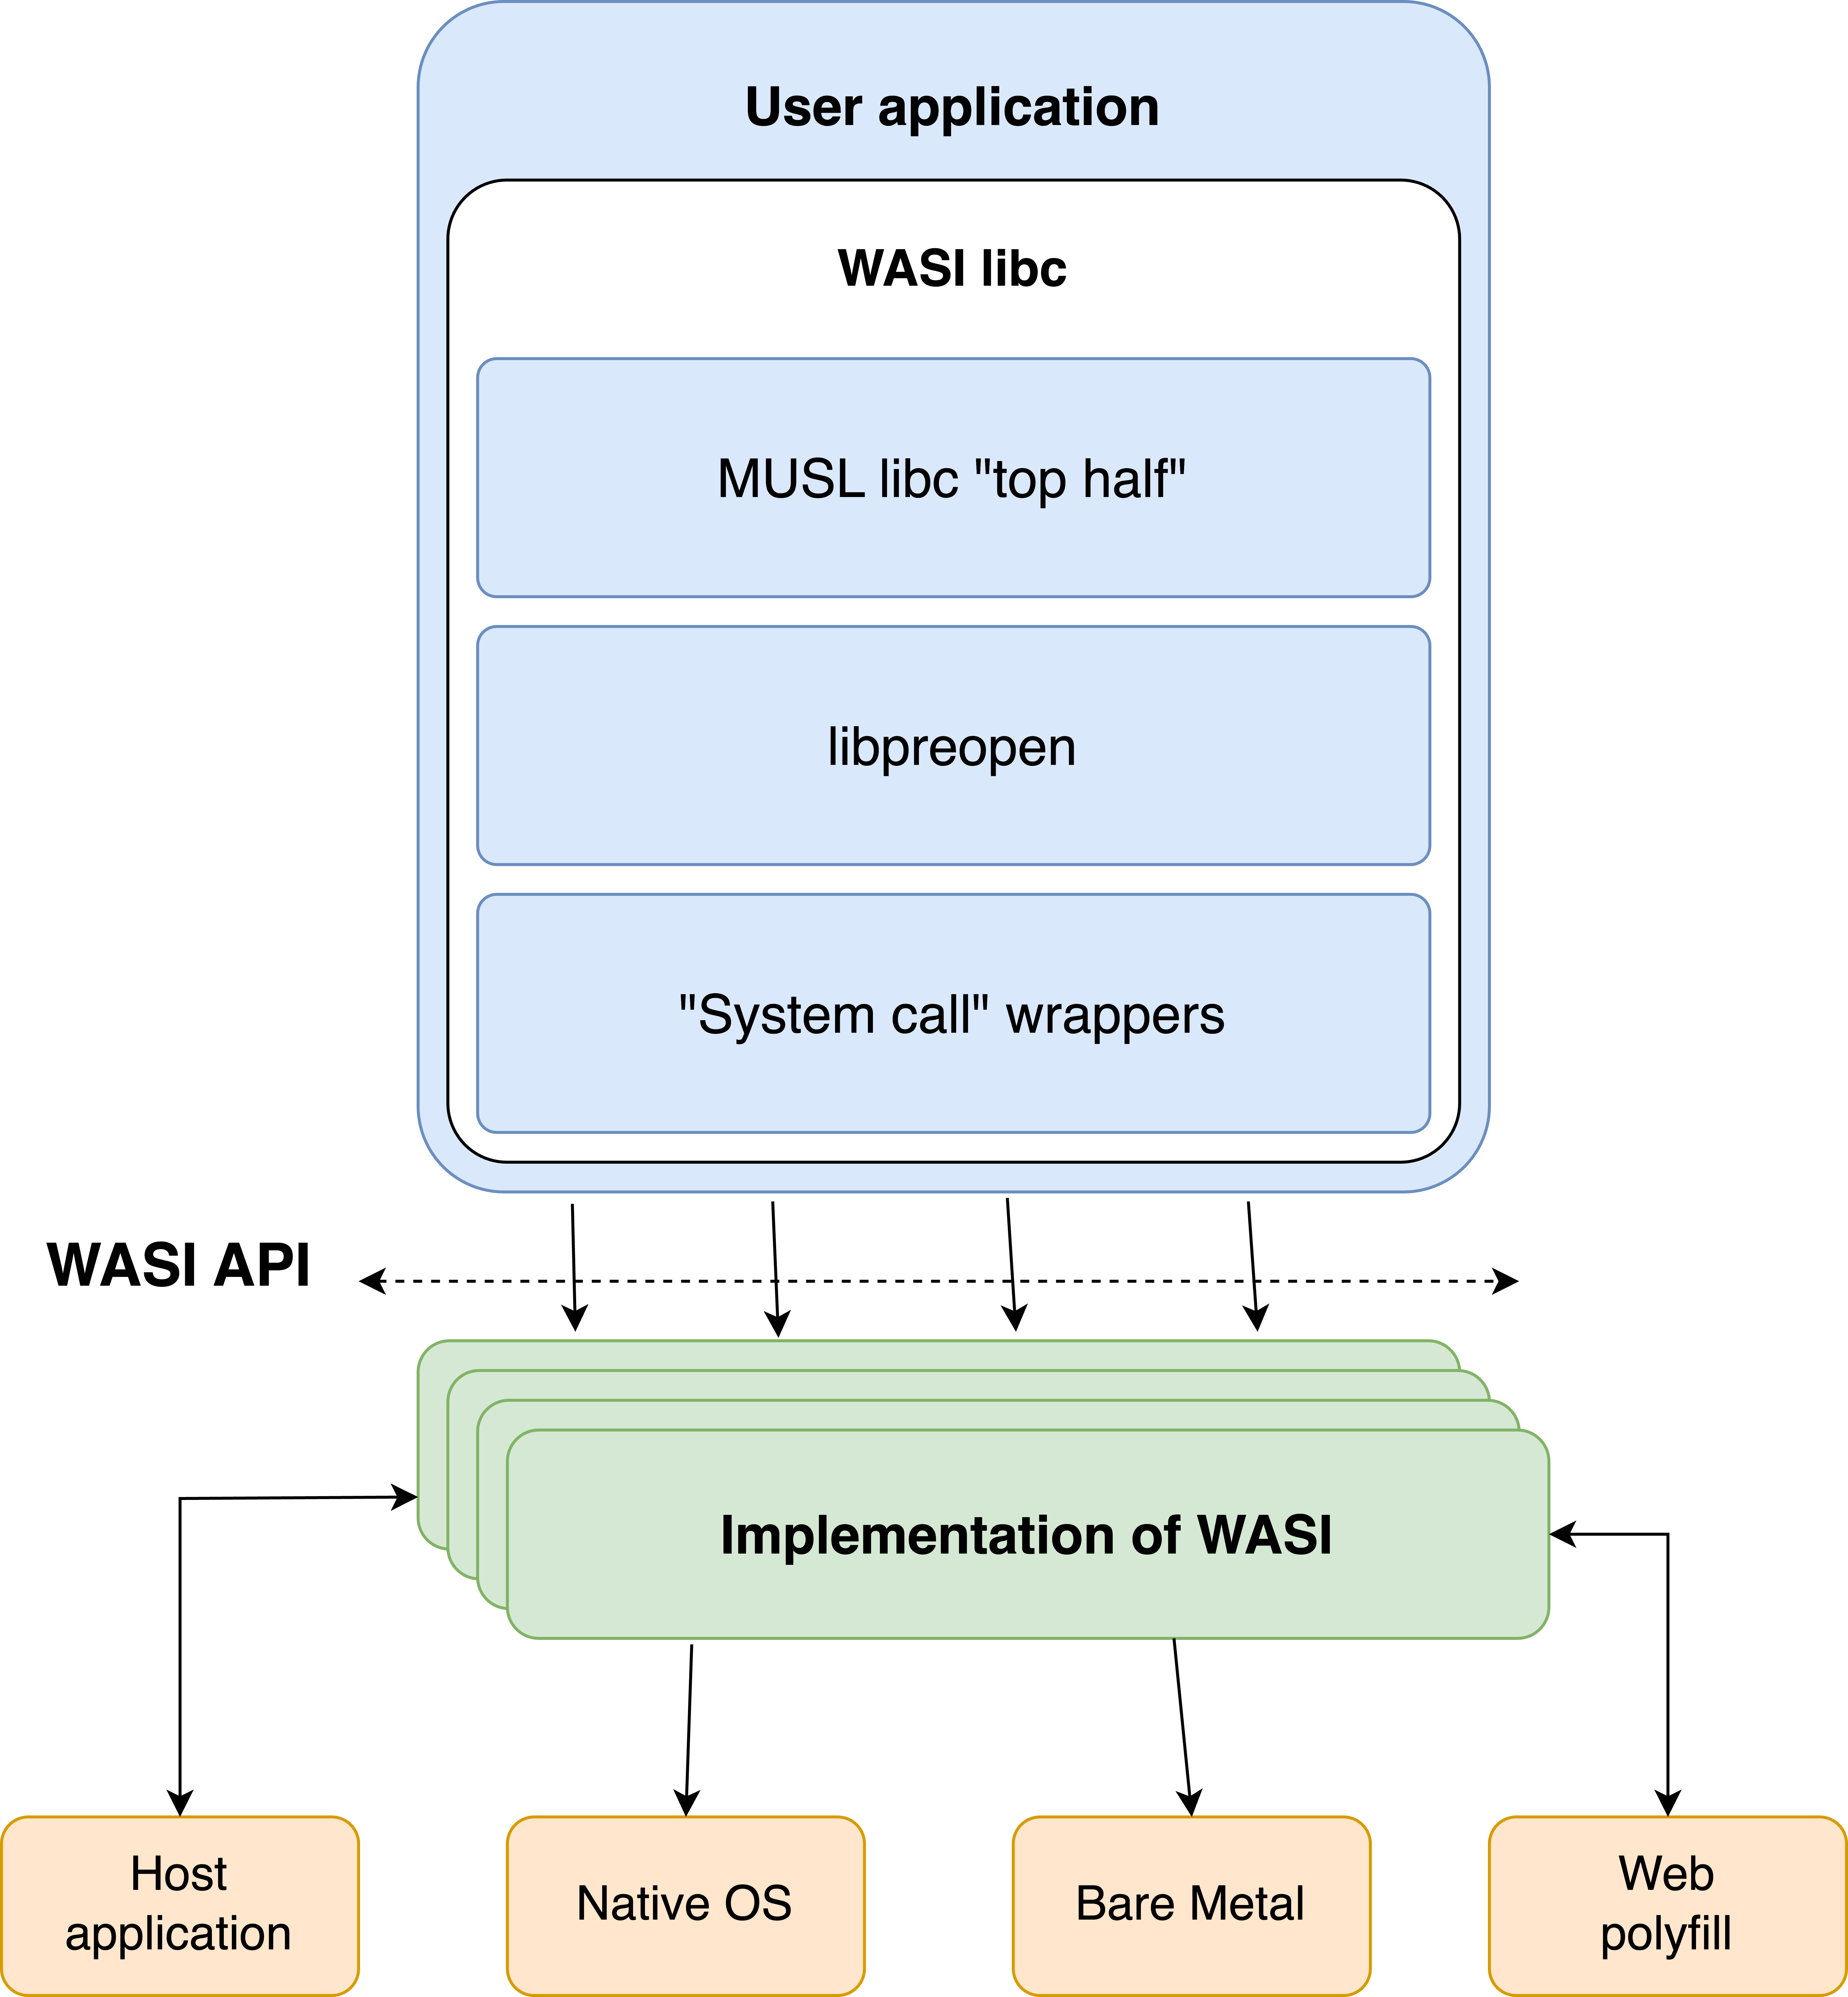
\includegraphics[width=130mm,scale=0.8]{images/wasm/WASI_Architecture.png}
	\caption{WASI Architecture}
	\label{fig:wasi-architecture}
\end{figure}

\subsection{WASI as Emscripten replacement?}
The first toolchain that enabled C, C++, or any other language with \gls{LLVM} support to be compiled into WebAssembly was Emscripten. Essentially, Emscripten can compile almost any portable C or C++ codebase into WebAssembly, encompassing high-performance games requiring graphics rendering, sound playback, and file loading and processing, as well as application frameworks like Qt. Emscripten has been utilized to convert numerous applications like Unreal Engine 4 and the Unity engine, into WebAssembly \cite{emscriptencommunity_2023_emscripten}. 

To achieve this, Emscripten implemented the \gls{POSIX} OS system interface on the web. 
As a result, developers are able to use the functions available in the C standard library (\gls{libc}). 
Emscripten accomplished this by creating its own implementation of libc, which was divided into two parts. One part was compiled into the WebAssembly module, while the other part was implemented in \gls{JS glue code}. 
The JS glue would subsequently communicate with the browser, which would in turn communicate with the Kernel and the OS.

\begin{figure}[H]
    \centering
        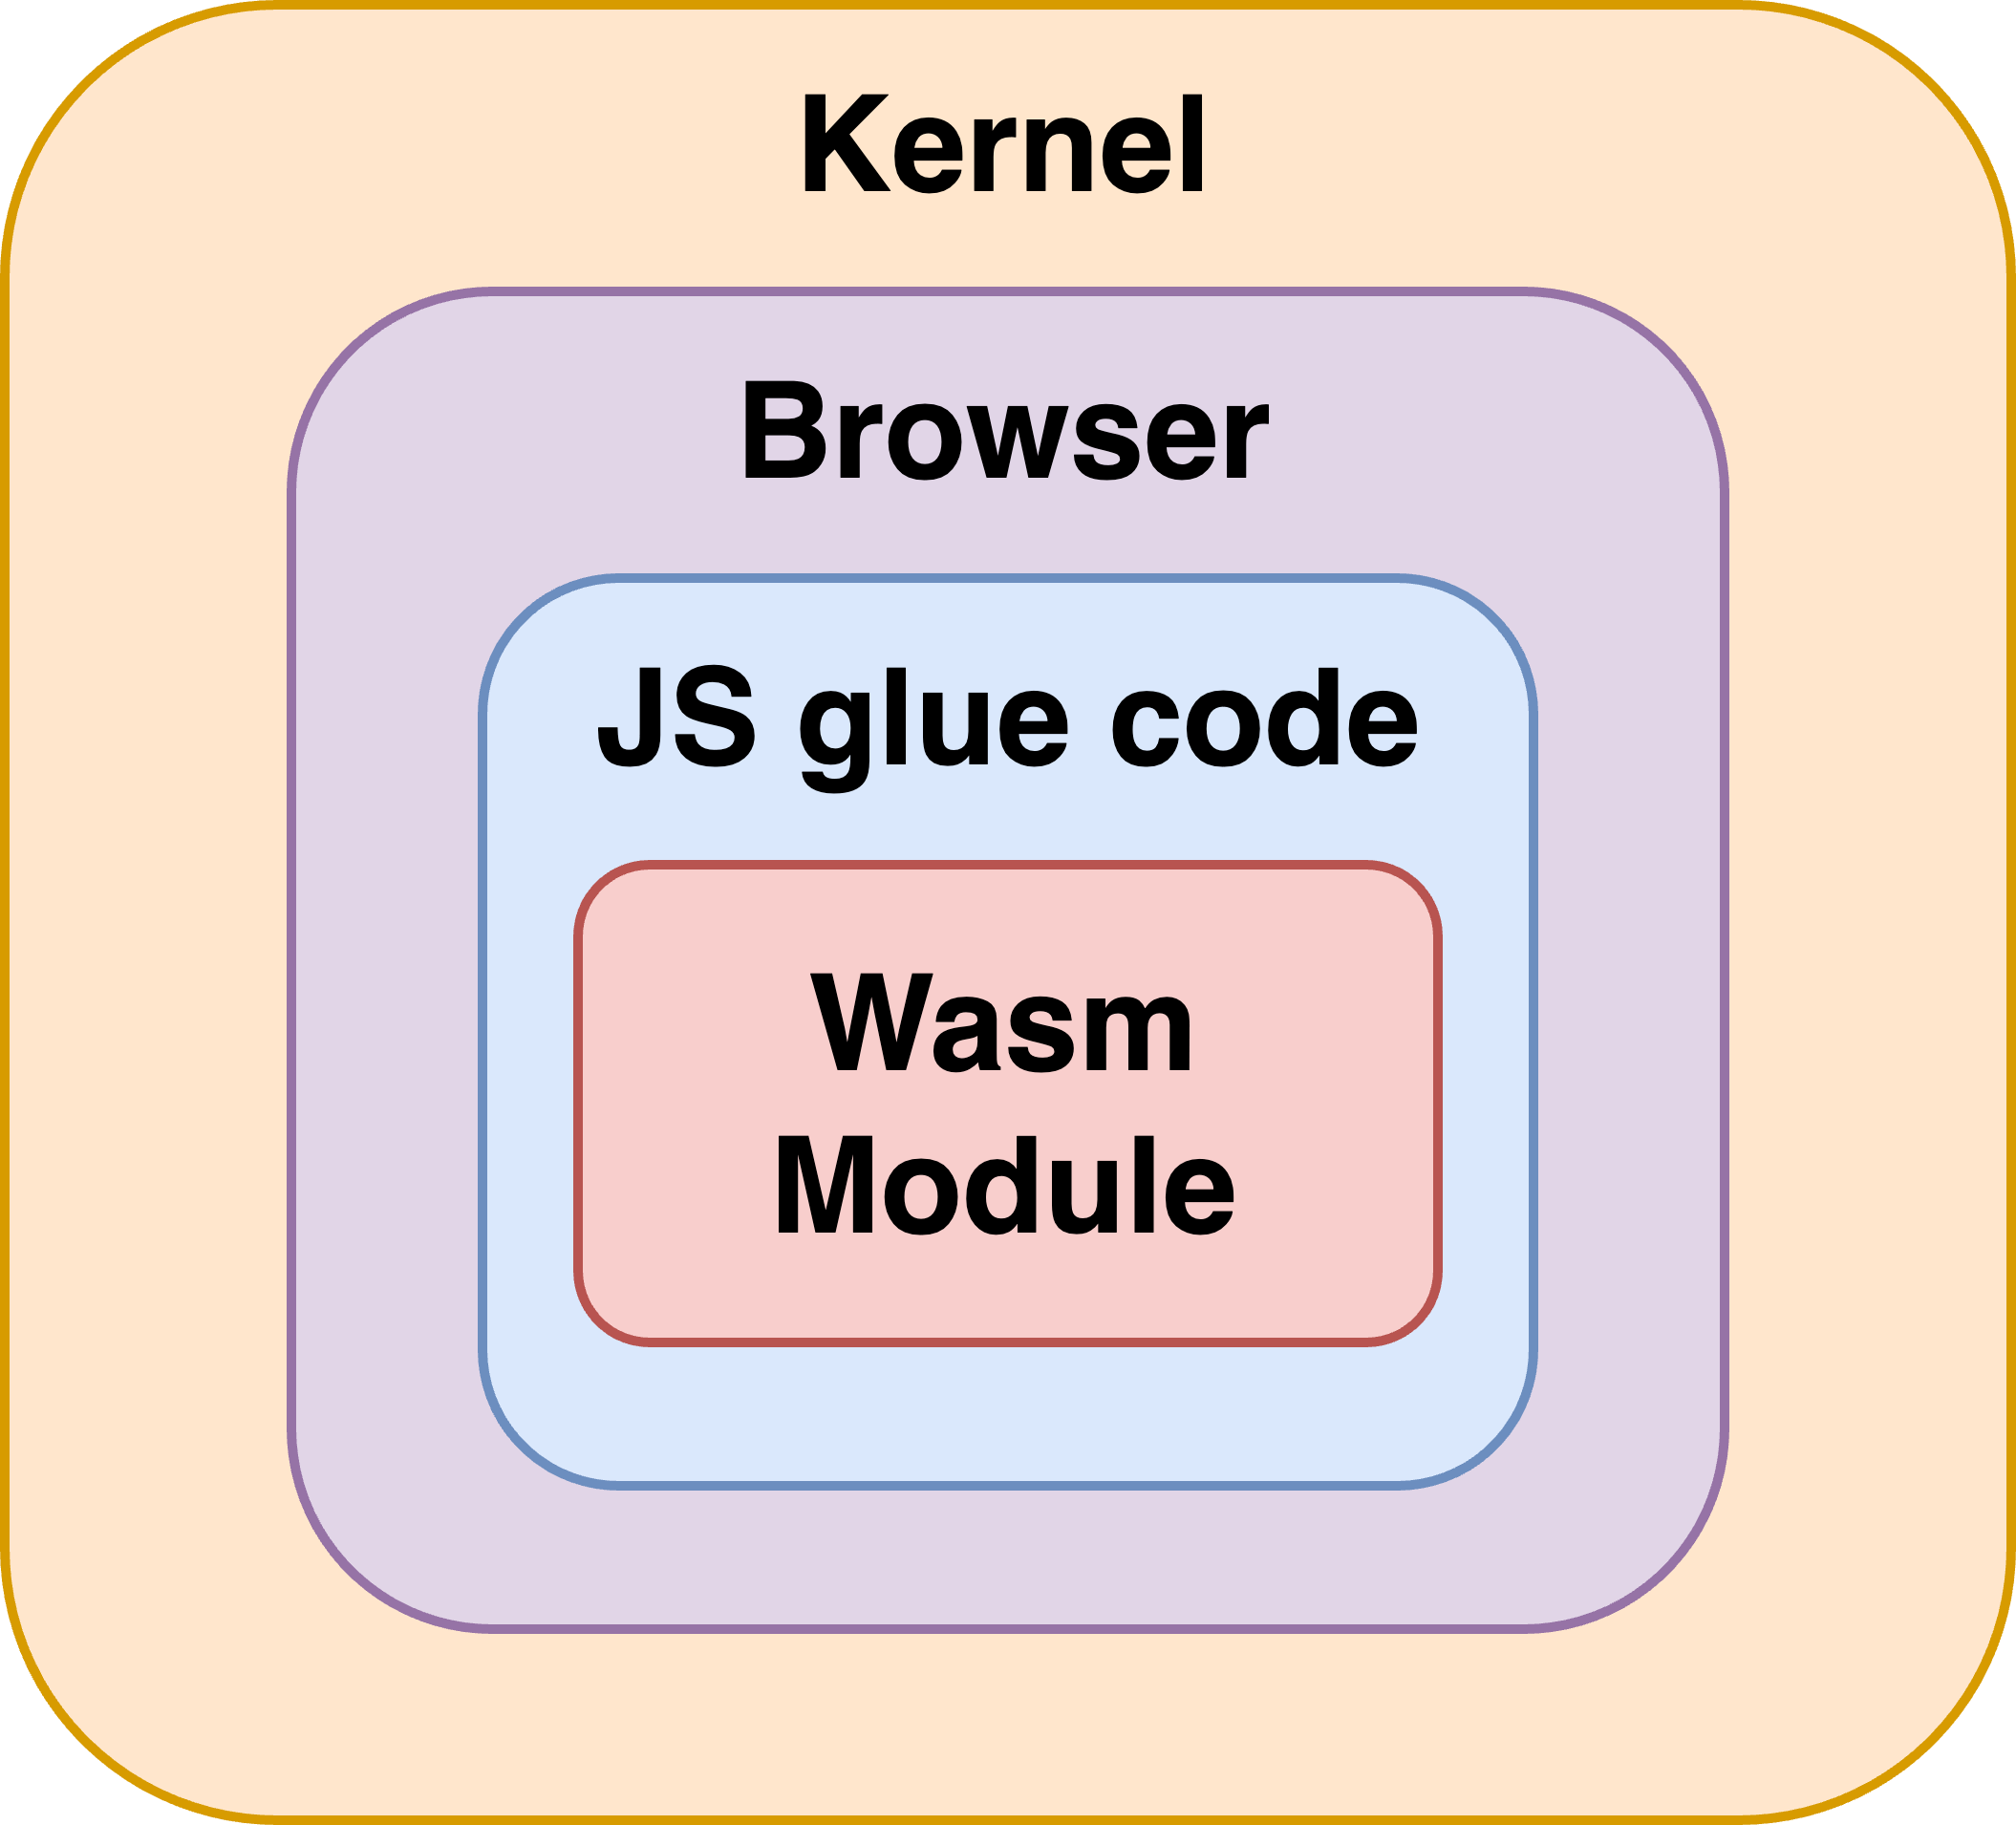
\includegraphics[width=0.6\linewidth]{images/wasm/Emscripten.png}
    \caption{Structure of Emscripten compiled Wasm module}
    \label{fig:emscripten}
\end{figure}

When users began to seek ways of running WebAssembly outside of a browser environment, the first approach was to enable the execution of Emscripten-compiled code on the corresponding environment.
To achieve this, the runtimes had to develop their own implementations of the functions in the JS glue code. However, this presented a challenge as the interface provided by the JS glue code was not intended to be a standard or public-facing interface. 
It was designed to serve a specific purpose, and creating a portable interface was not part of its intended design. The above figure \ref{fig:emscripten} shows the connection between the browser, the glue code and the Wasm module. 

Emscripten aims to improve the standard by using WASI APIs as extensively as possible in order to minimize unnecessary API differences. As previously stated, Emscripten code accesses Web APIs indirectly via JavaScript on the web. By making the JavaScript API resemble WASI, an unnecessary API difference can be eliminated, allowing the same binary to run on a server as well. In simpler terms, if a Wasm application wants to log information, it must call into JavaScript, following a process similar to this:

\verb|wasm => function musl_writev(...) { ... console.log(...) ... }|

"musl\_writev" represents an implementation of the Linux syscall interface utilized by "musl libc" to write data to a file descriptor, ultimately leading to a call to console.log with the appropriate data. The Wasm module imports and invokes "musl\_writev", thereby defining an ABI between the JavaScript and Wasm components. This ABI is arbitrary, by changing the existing ABI with one that aligns with WASI, the following can be achieved:

\verb|wasm => function __wasi_fd_write(...) { ... console.log(...) ... }|

% X 1. die API zu einem gewissen grad vereinheitlichen kann
% 2. es gibt dinge die emscripten machen kann aber wasi nicht macht
% 3. es macht vielleicht auch sinn eine api für web eine api für server und andere api's für plugins zu haben

%According to \cite{zakai_2019_outside} 

\subsection{WASI Portability}
\label{subsec:wasi-portability}

WebAssembly by design is a portable format, as mentioned before, the core specification does not make any platform specific assumptions. 
The first system API which the WASI community has been working on is the \gls{POSIX} API. 
It involves essential functionalities like file operations, processes, threads, 
shared memory, networking, regular expressions and so on. WASI will consist of a collection of low level and high level APIs, which aim to be as portable as possible. 

Figure \ref{fig:wasi-portability} illustrates that a source code can be compiled with different versions of libc to target various platforms. However, in the case of WASI, the same source code can be compiled into a portable binary that targets a virtual host platform called "wasm32-unknown-wasi". 
This target comprises three parts: the underlying architecture "wasm32", the vendor (which usually specifies the platform or hardware vendor; in this case, it is "unknown"), and the operating system ("wasi").

Comparing the left and right sides of the figure, we can observe that the Wasm binary runs on a WASI runtime, also known as a WASI engine. The implementation details of the underlying OS are abstracted away from the Wasm binary targeting WASI. For instance, suppose a small C program that opens a file, reads its contents, and prints them to the console. In that case, on a Linux system, the program would call the "open" syscall. 
However, on WASI, the program would call the "wasi\_fd\_open" function, which is part of the WASI API. 
The WASI module expects the engine to create a file descriptor and return it to the module, which it can then use to read the file contents.

\begin{figure}[H]
    \centering
        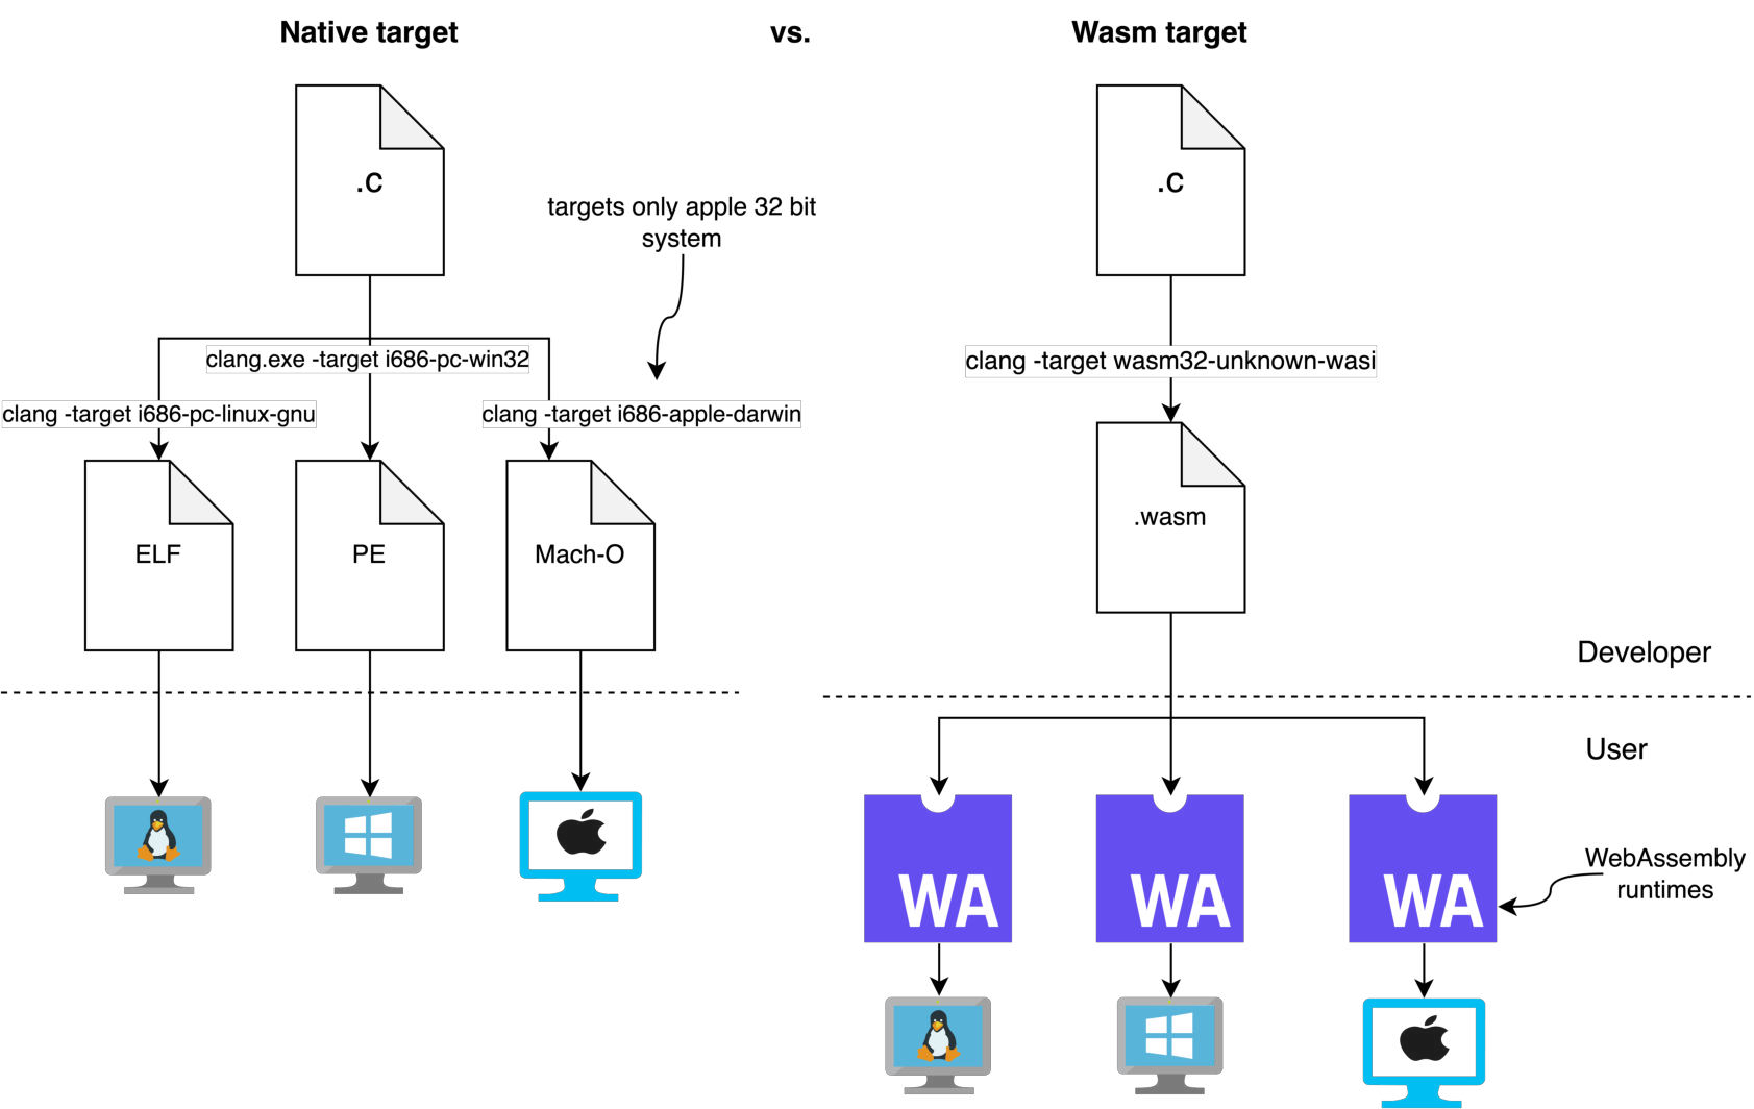
\includegraphics[width=1\linewidth]{images/wasm/WASI_PORTABILITY.pdf}
    \caption{WASI portability model redrawn from \cite{clark_2019_standardising}}
    \label{fig:wasi-portability}
\end{figure}

Aside from the information provided in Figure \ref{fig:wasi-portability}, it should be noted that because of WASI's portability, the modules are not confined to a particular host platform. They have the flexibility to be integrated into an application, function as a plugin, or run as a serverless function in the cloud, as referenced in \cite{clark_2022_wasmtime}, as long as the host runtime supports the required APIs.

\subsection{WASI Security Model}
\label{subsec:wasi-security-model}

An essential aspect of any system is the security model implemented to ensure the integrity and confidentiality of data and resources. When a code segment requests the operating system (OS) to perform input or output operations, the OS must ascertain whether the action is secure and permissible.

Operating systems generally employ an access control mechanism based on ownership and group associations to manage security. For instance, consider a scenario where a program seeks permission from the OS to access a specific file. Each user possesses a unique set of files they are authorized to access. In Unix systems, for example, the ownership of a file can be assigned to three classes of users: user, group, and others.

Upon initiating the program, it operates on behalf of the respective user. Consequently, if the user has access to the file—either as the owner or as a member of a group with access rights—the program inherits the same privileges. This approach to security helps maintain a robust and reliable system that adheres to the principles of access control and resource protection.

This approach was effective in multi-user systems where administrators controlled software installation, and the primary threat was unauthorized user access. However, in modern single-user systems, the main risk comes from the code that the user runs, which often includes third-party code of unknown trustworthiness. This raises the risk of a supply chain attack, particularly when new maintainers take over open-source libraries, as their unrestricted access could enable them to write code that compromises system security by accessing files or sending them over the network \cite{clark_2019_standardising}.

 % explain supply chain attack

The security aspect of WASI is vital to the universal nature of WebAssembly. The WASI standard was built on a capabilities-based security model, which means the host has to explicitly permit capabilities such as file system access and establishing network sockets. As a result, a WASI module cannot run arbitrary code with direct access to memory.

In the context of serverless computing, for instance, a cloud provider may allow or deny access to specific functions, thus implementing security policies on a per-function basis. However, this level of granularity may not be sufficient. Since WebAssembly does not employ virtualization, all modules share common resources, such as the file system. As a result, the cloud provider may want to permit serverless functions to temporarily cache data in a specific "/tmp/<unique-id>/" directory while forbidding access to confidential files like "/etc/passwd". This is where WASI incorporates concepts from capability-based security.
